\chapter{Proposta}

\section{Requisitos Funcionais}
\subsection{Estórias de Usuário}
\textbf{US1 - Expert Correlação Linear}

Como pesquisador, gostaria de usar o método de Correlação de Pearson para verificar sua eficácia no Mercado de Moedas.

Critérios de aceitação US1:
\begin{itemize}
\item A Correlação de Pearson deve ser maior que 0.8 e o mercado estar subindo para se realizar a venda;
\item A Correlação de Pearson deve ser maior que 0.8 e o mercado estar caindo para se realizar a compra;
\item O take profit e o stop loss devem ser os mesmos.
\end{itemize}

\textbf{US2 - Expert Fibonacci}
Como pesquisador, gostaria de usar o método de Fibonacci para verificar sua eficácia no Mercado de Moedas.

Critérios de aceitação US2:
\begin{itemize}
\item Na situação em que o mercado estiver caindo e a regressão de Fibonacci estiver em 0.62, deve-se apenas vender no mercado com take profit e stop loss em 500 pontos;
\item Na situação em que o mercado estiver subindo e a regressão de Fibonacci estiver em 0.62, deve-se apenas comprar no mercado com take profit e stop loss em 500 pontos.
\end{itemize}

\textbf{US3 - Expert Mínimos Quadrados}

Como pesquisador, gostaria de usar o método de Mínimos Quadrados para verificar sua eficácia no Mercado de Moedas.

Critérios de aceitação US3:
\begin{itemize}
\item Não deve existir stop loss ou take profit fixos, pois os mesmos são variáveis de acordo com a estratégia do método de Mínimos Quadrados;
\item O método deve seguir a tendência do mercado. Se o mercado estiver subindo, deve-se comprar e se estiver caindo, deve-se vender.
\end{itemize}

\textbf{US4 - Expert Estocástico}

Como pesquisador, gostaria de usar o método de Estocástico para verificar sua eficácia no Mercado de Moedas.

Critérios de aceitação US4:
\begin{itemize}
\item Com estocástico acima de 0.80, deve-se vender com stop loss e take profit em 500 pontos;
\item Com estocástico acima de 0.20, deve-se comprar com stop loss e take profit em 500 pontos.
\end{itemize}

\textbf{US5 - Expert Média Móvel}

Como pesquisador, gostaria de usar o método de Média Móvel para verificar sua eficácia no Mercado de Moedas.

Critérios de aceitação US5:
\begin{itemize}
\item Se a média móvel lenta (12), cruzar a média rápida (26) de baixo para cima, deve-se comprar;
\item Se a média móvel lenta (12), cruzar a média rápida (26) de cima para baixo, deve-se vender.
\end{itemize}

\section{Arquitetura do Projeto}

Por usar vários paradigmas a ferramenta terá vários módulos, cada módulo com seu paradigma e responsabilidade, como mostrado na figura \ref{componente}.

\begin{figure}[htp]
\centering
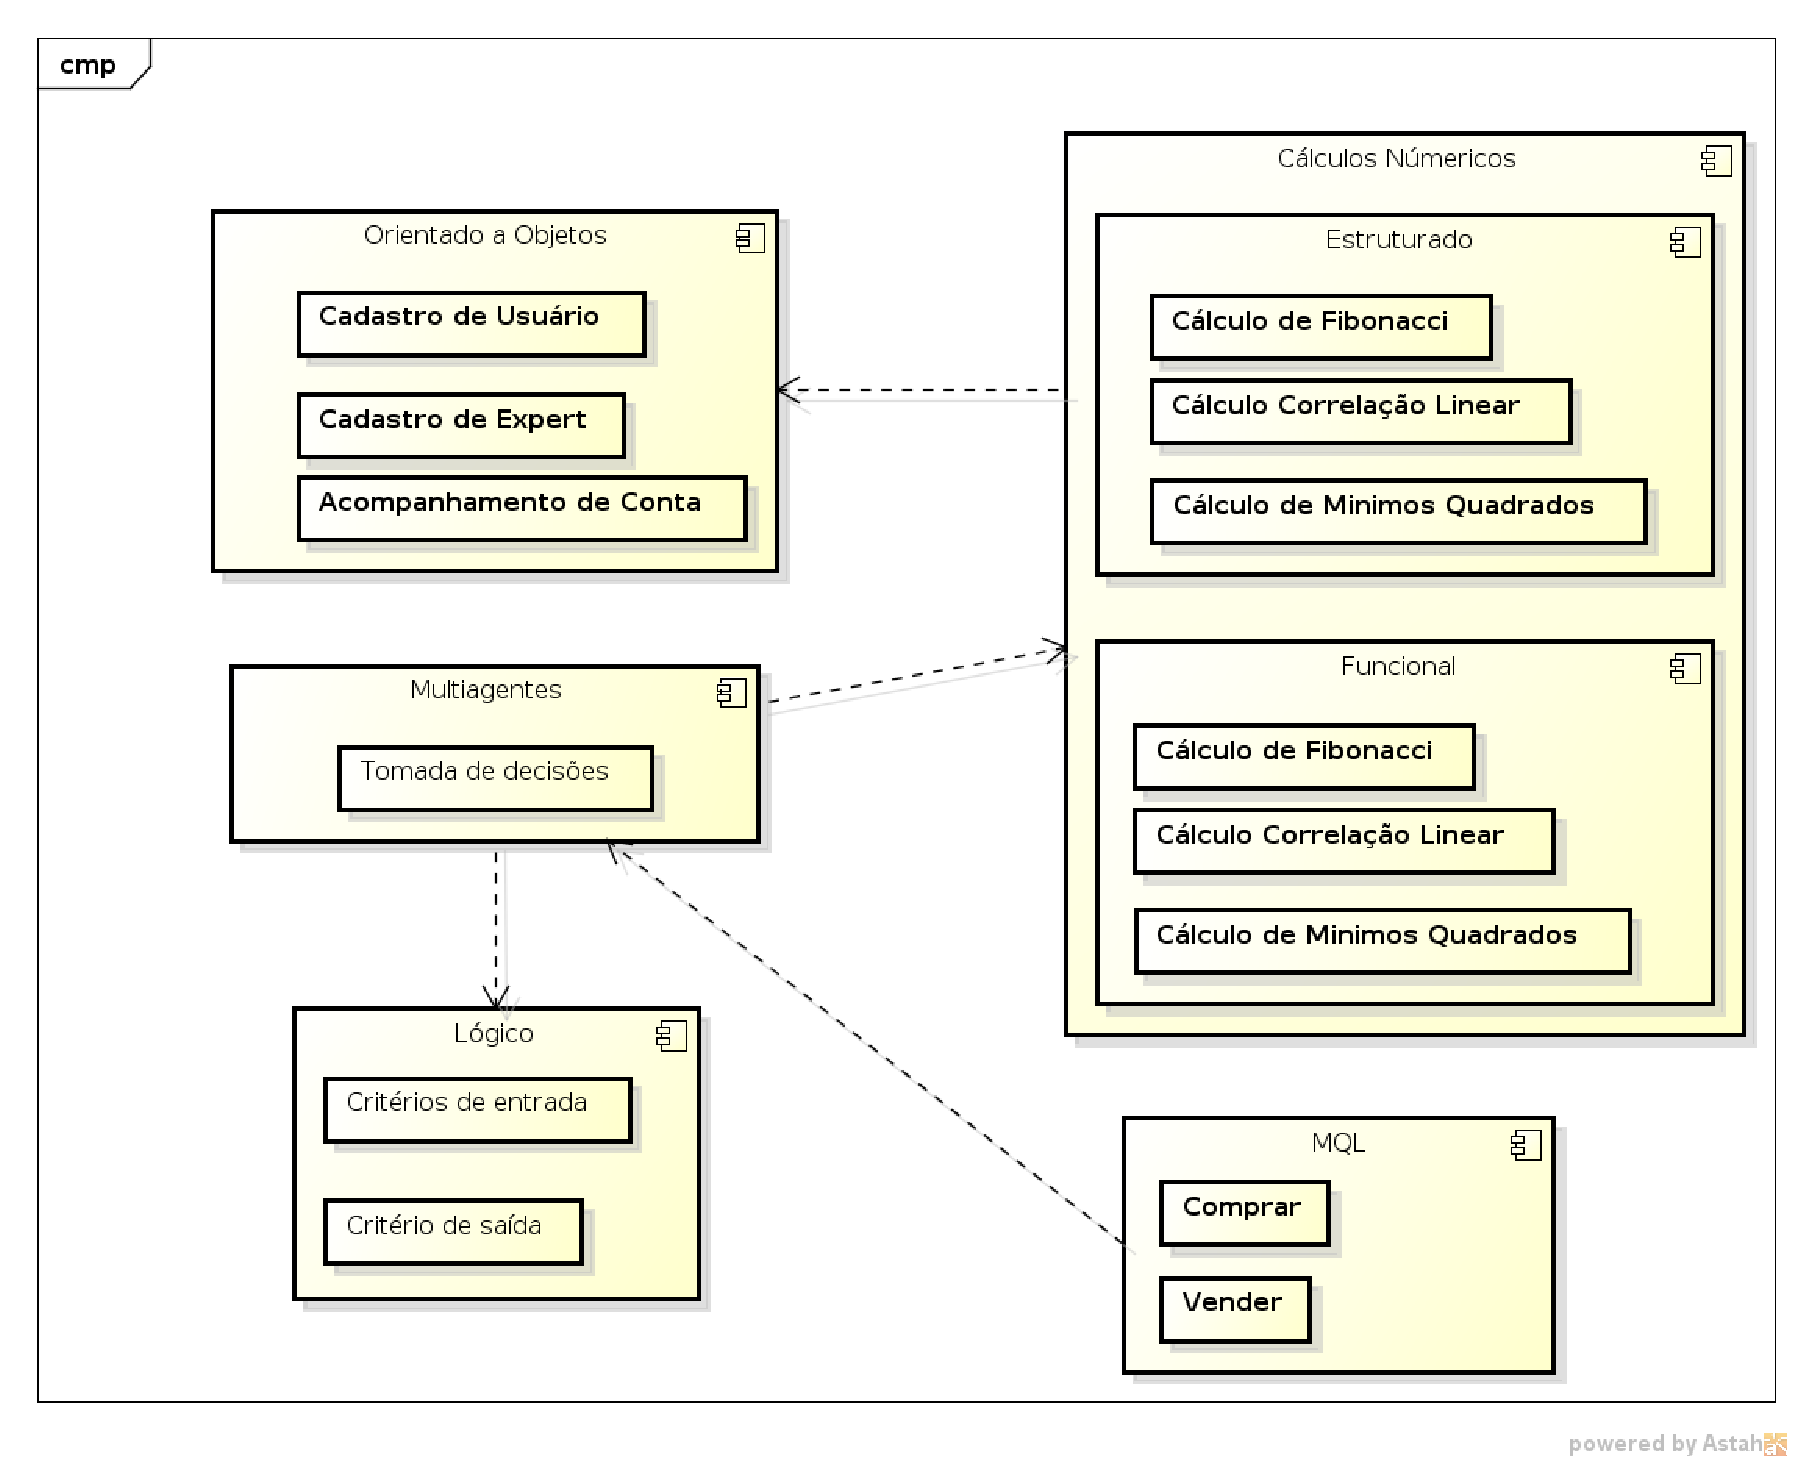
\includegraphics[width=0.9\textwidth]{figuras/componente}
\caption{Diagrama de Componente do Invest MVC}{Fonte: Autores} 
\label{componente}
\end{figure}

O módulo groovy fará a interação com o usuário. A escolha da linguagem de programação Groovy se deu porque esta é voltada para aplicações web e juntamente com  o framework grails, fornece na criação do projeto uma arquitetura MVC definida. Esta linguagem de programação é orientada a objetos, essa razão permite uma abstração do mundo, desta forma foi escolhido para  criação do site, uma vez que é preciso que uma entidade represente os usuários e seus experts.

O módulo Cálculos Numéricos será responsável por realizar os métodos matémáticos presentes na ferramenta Invest MVC, este módulo é composto por dois outros módulos: módulo C e módulo Haskell.

Haskell é uma linguagem de programação funcional, uma vez que sua "gramática" está proóxima das funções matemáticas, a implementação de funções matemáticas, métodos algébricos e numéricos se torna intuitiva quando se usa programação funcional. Além do mais este paradigma é declarativo, por limitar o uso de atribuições à variáveis suas funções são mais precisas do que em outros paradigmas. Por isso o paradigma funcional foi eleito para implementar os métodos matemáticos.

Já a linguagem de programação C é estruturada, …

O módulo Controle de comportamento será implementado usando Multi-Agentes. Considerando que os agentes de software são entidades autonomas e com capacidades socias. O uso deste paradigma justifica-se na tomada de decisões ( compra e venda de moedas). Pois sua  caracteristica autônoma dispensa a presença de um usuário interagindo com sistema. Os agentes MVC possuem uma arquitetura reativa, suas ações se dão por "mudanças" que ocorrem no  mercado de moedas.

O módulo Base de conhecimento será produzido em Prolog, uma linguagem de programação lógica,  uma vez que este  paradigma facilita a representação, inserção e recuperação de conhecimento.

Na Figura \ref{componente} é possível perceber que os módulos interagem entre sim, essa interação fica mais evidente no diagrama de sequência do sistema, figura \ref{sequencia}.

\begin{figure}[htp]
\centering
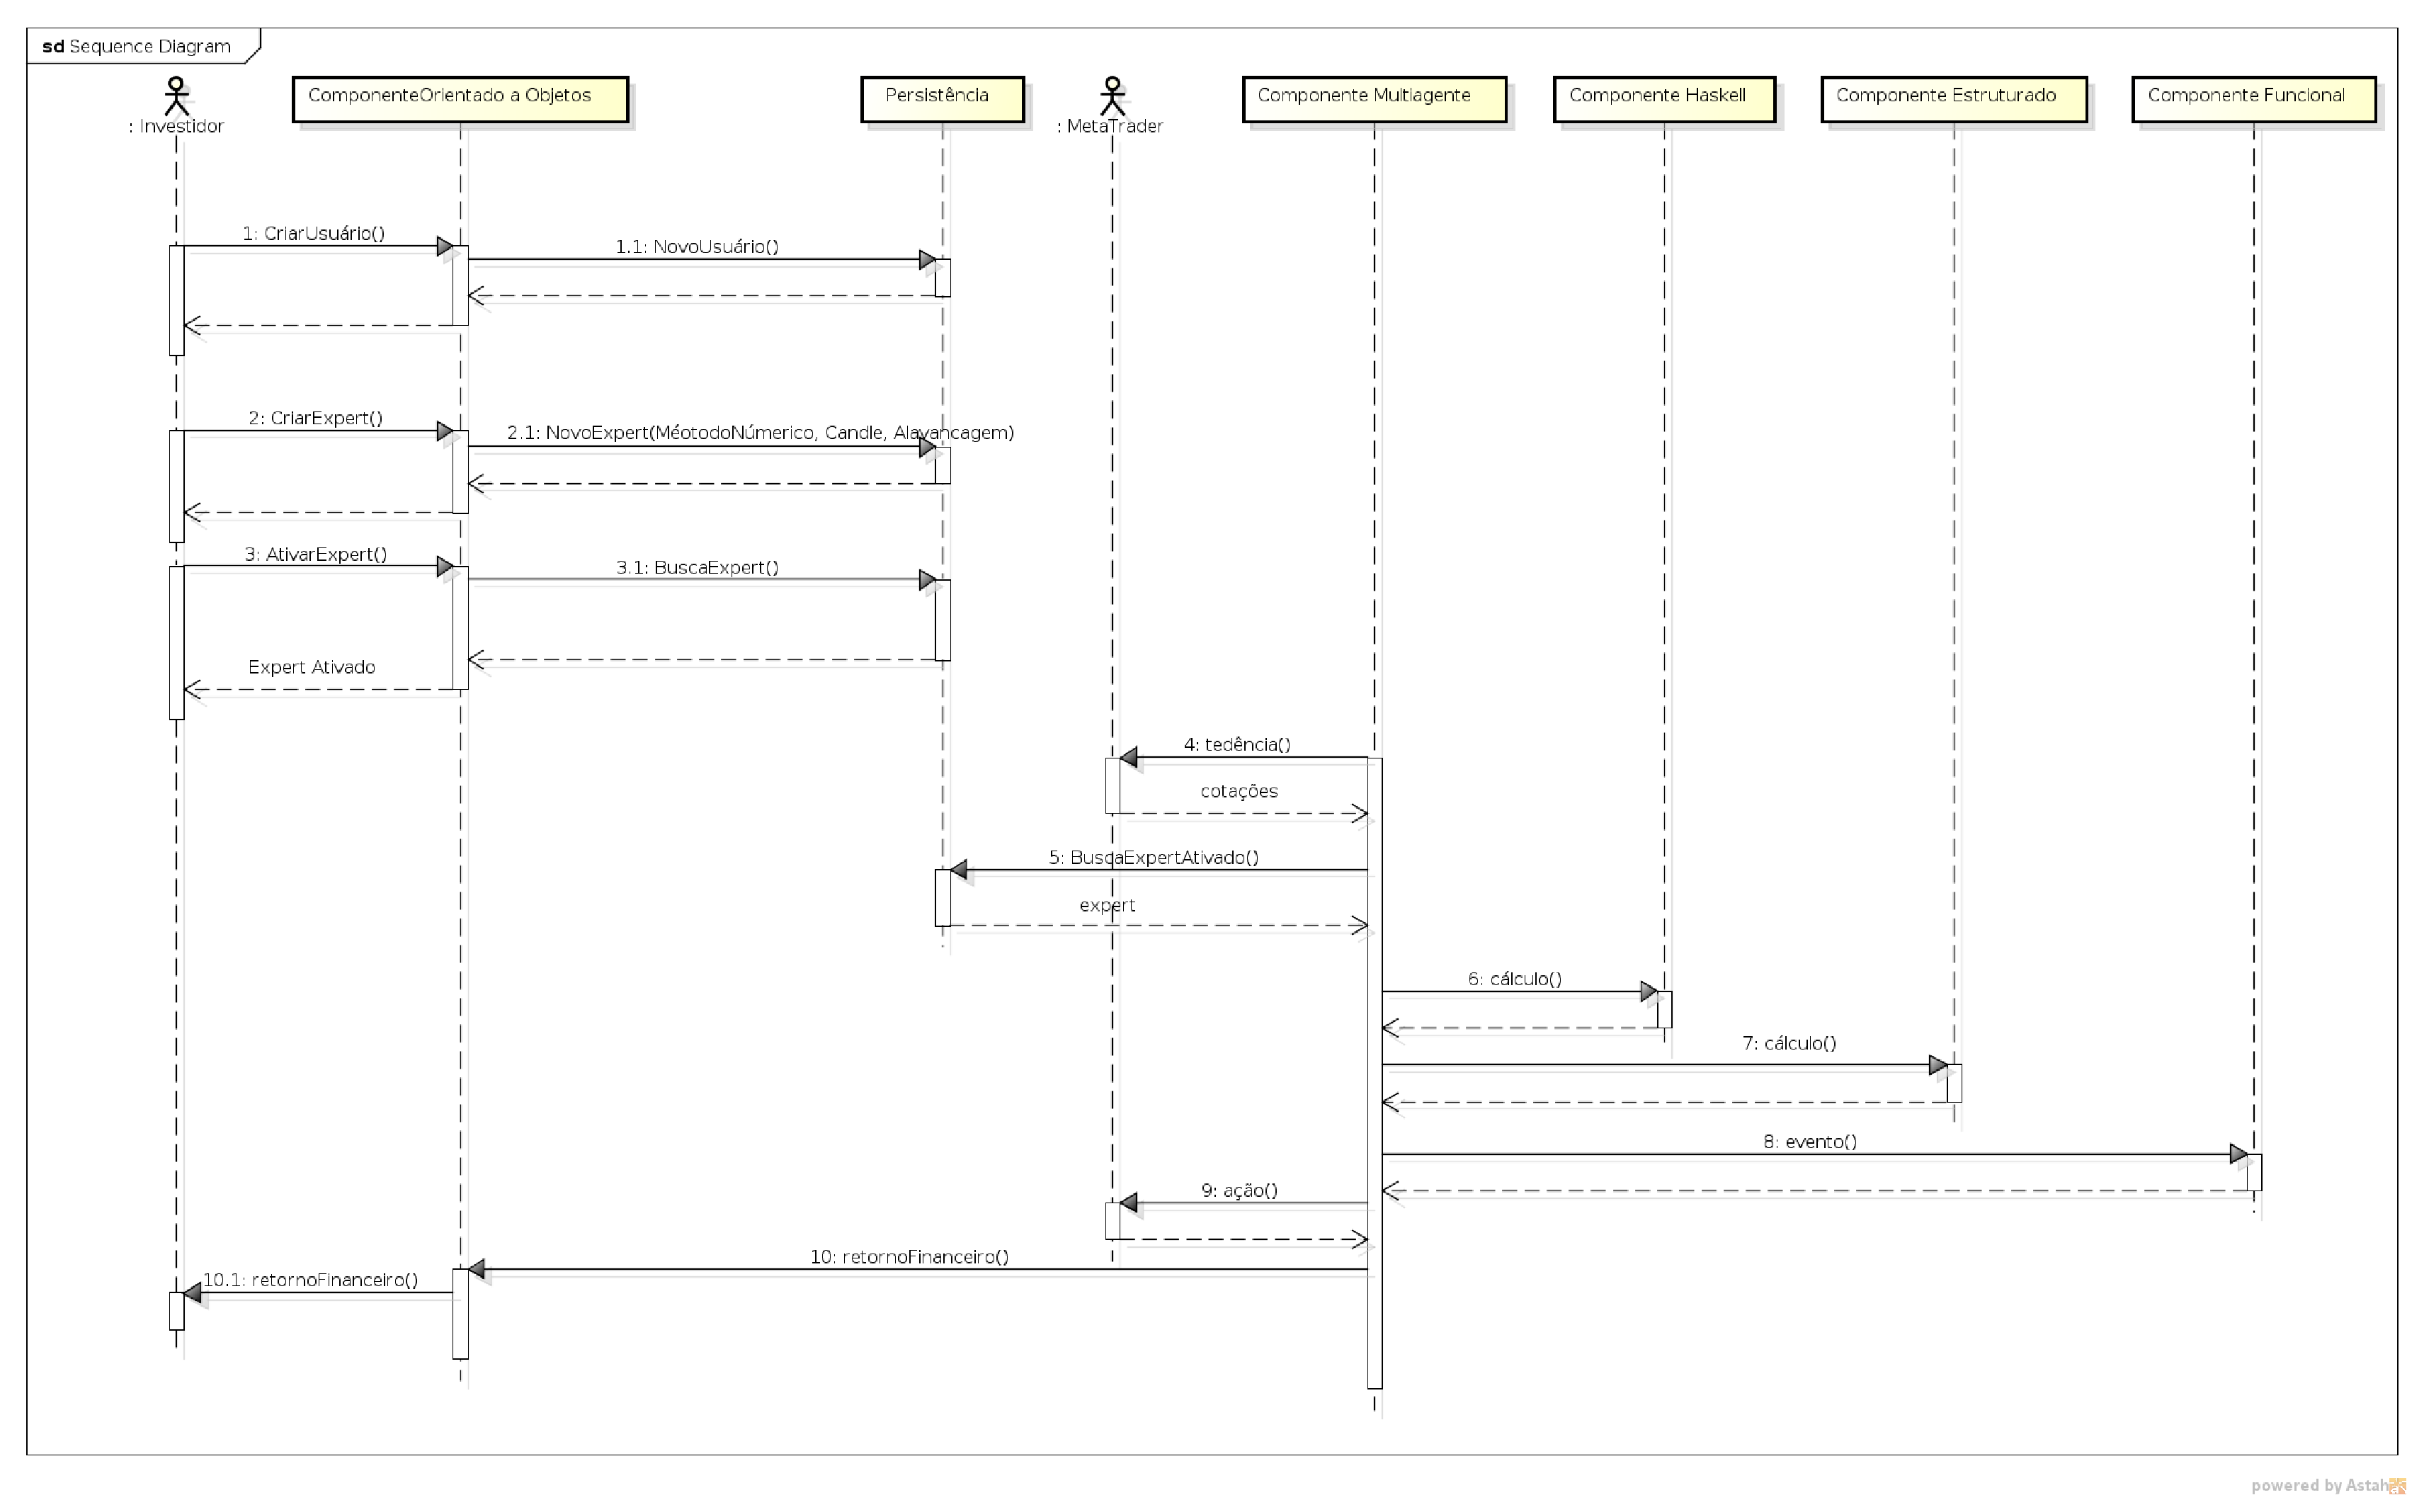
\includegraphics[width=0.9\textwidth]{figuras/sequencia}
\caption{Diagrama de Sequência do Invest MVC}{Fonte: Autores} 
\label{sequencia}
\end{figure}

O investidor interage apenas com o módulo Groovy, criando seu usuário e experts, no qual serão persistidos. O investidor também poderá ativar um expert.
O módulo Multi-agentes vai verificar a tedência do mercado de moedas, por meio da plataforma Meta-Trader. Logo o módulo Multi-Agentes buscará na persistência o expert que está ativo. Sabendo qual método matemático o expert foi cadastro, o módulo multi-agente faz a requisição de cálculos para os módulos C e Haskell. A partir desse resultado o sistema Multi-agentes procurará no Módulo prolog, eventos análogos. Caso exista tais eventos análogos ao que ocorre, o módulo multi-agentes decidirá entrar no mercado para tomar ações(compra ou venda) com mais investimento.
